\DeclareRobustCommand{\figExample}{%
\begin{figure}[t]
    \centering
    \resizebox{\linewidth}{!}{%
    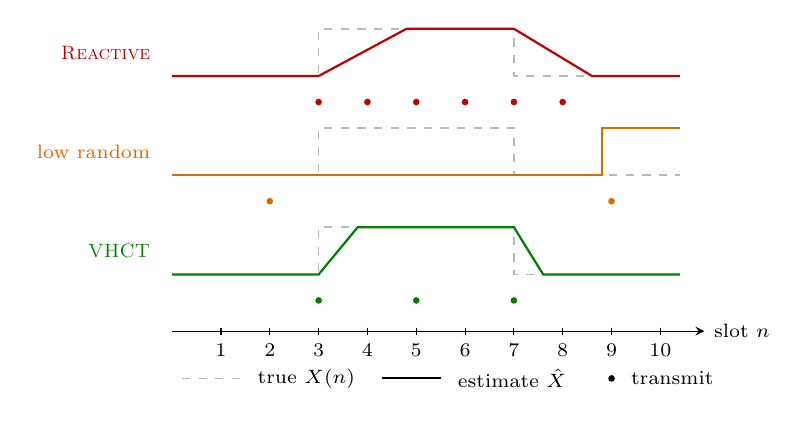
\begin{tikzpicture}[x=0.62cm, y=0.30cm, font=\scriptsize, >=stealth,
        sig/.style={thick},
        truth/.style={gray!55, dashed, line width=0.6pt},
        tx/.style={circle, inner sep=0pt, minimum size=2.4pt, draw=none}]
        % one lane per policy: the true signal (dashed) against that policy's
        % estimate (solid), with the slots it chose to transmit in underneath
        \foreach \base in {0, 4.2, 8.4} {
            \draw[truth] (0,\base) -- (3,\base) -- (3,\base+2)
                      -- (7,\base+2) -- (7,\base) -- (10.4,\base);
        }
        % reactive: reacts to every error, six transmissions
        \draw[sig, red!75!black] (0,8.4) -- (3,8.4) -- (4.8,10.4)
                              -- (7,10.4) -- (8.6,8.4) -- (10.4,8.4);
        \foreach \n in {3,4,5,6,7,8} \node[tx, fill=red!75!black] at (\n,7.3) {};
        \node[anchor=east, red!75!black] at (-0.25,9.4) {\textsc{Reactive}};
        % a sparse fixed rate: misses the first jump entirely
        \draw[sig, orange!85!black] (0,4.2) -- (8.8,4.2) -- (8.8,6.2) -- (10.4,6.2);
        \foreach \n in {2,9} \node[tx, fill=orange!85!black] at (\n,3.1) {};
        \node[anchor=east, orange!85!black] at (-0.25,5.2) {low random};
        % learned: tracks both changes with three transmissions
        \draw[sig, green!50!black] (0,0) -- (3,0) -- (3.8,2)
                                -- (7,2) -- (7.6,0) -- (10.4,0);
        \foreach \n in {3,5,7} \node[tx, fill=green!50!black] at (\n,-1.1) {};
        \node[anchor=east, green!50!black] at (-0.25,1.0) {\textsc{VHCT}};
        % shared slot axis
        \draw[->] (0,-2.4) -- (10.9,-2.4) node[right] {slot $n$};
        \foreach \n in {1,...,10} \draw (\n,-2.25) -- (\n,-2.55) node[below=0pt] {\n};
        % what the dashing and the triangles mean
        \draw[truth] (0.2,-4.4) -- (1.4,-4.4);
        \node[anchor=west] at (1.55,-4.4) {true $X(n)$};
        \draw[sig, black] (4.3,-4.4) -- (5.5,-4.4);
        \node[anchor=west] at (5.65,-4.4) {estimate $\hat{X}$};
        \node[tx, fill=black] at (9.0,-4.4) {};
        \node[anchor=west] at (9.2,-4.4) {transmit};
    \end{tikzpicture}%
    }
    \caption{Motivating example on one sensor over ten slots. \textsc{Reactive} sampling reacts to every error but transmits six times; a sparse random policy misses the first jump; \textsc{VHCT} transmits three times and tracks both changes.}
    \label{fig:overview-example}
\end{figure}%
}
